% -- choice of grid search vs. MCMC, and NN-based acceleration
% -- method validation with simulated photometry
% -- distance scale validation with SDSS-Gaia Stripe 82 sample 
% -- 3D dust map derived from SDSS data in Galactic plane 
% 
%   for spinoff papers: 
%      -- kuglasti skupovi
%      -- aginst Rich et al. BDSD survey ugriz podaci

\section{Numerical Implementation and Performance Tests \label{sec:tests}}

We first discuss our numerical implementation choices and then test the method's performance using simulated TRILEGAL catalogs. We
validate adopted luminosity-color models and implied distance scale using SDSS and Gaia observations. An all-sky pipeline implementation
and its performance are discussed in the next Section. 

\subsection{Accelerated Exhaustive Grid Search Method}

Luminosity-color models introduced in \S\ref{sec:method} are expressed as lookup tables, rather than as analytic functions. They are initially defined
on a two-dimensional grid, and after accounting for dust extinction, on a three-dimensional grid. We use equidistant grids for all three
model parameters: 0.01 mag for $M_r$, 0.05 dex for $[Fe/H]$ and a range of steps from 0.005 mag to 0.02 mag for $A_r$, depending on its
prior range. These grids have sufficient resolution for numerical analysis of the posterior probability distributions and typically
result (depending on the maximum allowed $A_r$ value) in several
million grid points. For a given star, the exhaustive grid search method simply iterates
over all these points and for each computes likelihood and ultimately the posterior pdf. 

Significant acceleration can be achieved by using a two-step iteration, with degraded grids in the first step, but still fine
enough to sufficiently resolve the posterior pdf to approximately estimate its behavior around its maximum. We find that degrading the
$M_r$ step to 0.05 mag and the $[Fe/H]$ step to 0.1 dex works well in practice and results in a about ten times shorter run time. After the first iteration, the range $\pm 3
\sigma$ around the posterior  maximum, where $\sigma$ is standard deviation, is estimated using the marginal distribution for each model
parameter. The calculation of the posterior is then repeated using the finest grid but only in the $\pm 3 \sigma$  neighborhood
(cube) around the posterior maximum, which includes 100 to 1000 times fewer grid locations. 

With this acceleration trick, runtime per star is typically about 10 millisec per star  (it varies nearly proportionally to the maximum allowed $A_r$ value). 
While exceedingly simple, this method is sufficiently fast and robust to offer a convenient practical solution for processing samples of billions of stars. 


\subsubsection{Markov Chain Monte Carlo Method}
 
Markov Chain Monte Carlo methods have been successfully used in this context (e.g., \citealt{2014ApJ...783..114G}). 
Given that we aim to process LSST photometry for about 10$^{10}$ stars, it is worthwhile to compare the MCMC runtime
to the runtime for our accelerated exhaustive grid search method. We considered two implementations, based on {\it PyMC3} \citep{pymc2023} and
{\it emcee} \citep{2013PASP..125..306F}. The latter was about 10-20 times faster than the former; for example, with 4 ``walkers'' and 500
iterations, it took on average about 0.1 sec per star. Therefore, in this low-dimensional case (there are only three model parameters) the
grid search method described above is about an order of magnitude faster than the {\it emcee} implementation. 


\subsubsection{Neural Network Method}

Further acceleration can be achieved using the Neural Network method. In a companion paper by Mrakov\v{c}i\'{c} et al., we describe
how to use a small subsample of stars to train a neural network model and then estimate model parameters and their uncertainty for the remaining
stars using the trained network. This approach yields runtimes of about 1 milisec per star, that is, shorter by an order of magnitude than when
the grid search method is used for the full sample. With this additional speed up, a sample of 10 billion stars can be processed in
about 10 hours using a 300-core machine and the pipeline described in the next Section. 


\subsection{Performance Testing} 

We first validate numerical implementation of our method using a simulated dateset, where the true model parameters are known.
The luminosity-color model tracks are then validated using SDSS photometry from the so-called Stripe 82 region and trigonometric
distances obtained using Gaia data. Finally, we demonstrate
performance in the large $A_r$ regime and three-dimensional mapping of interstellar dust distribution using SDSS
scans that cross high-extinction regions in the Galactic plane.
 

\subsubsection{Simulated Data Set}
 
Our simulated catalogs are based on TRILEGAL simulations of LSST stellar content by \cite{2022ApJS..262...22D}, already
mentioned in the context of priors in \S\ref{sec:priors}. We use these simulations to generate distributions in the
$M_r$--$[Fe/H]$--$A_r$--magnitude--sky position space. Given these quantities for a sample of simulated TRILEGAL stars,
we generate simulated LSST photometry for each star as follows: 
\begin{enumerate}
\item
Given relevant model parameters (e.g., $M_r$ and $[Fe/H]$ for main sequence and red giant stars, $M_r$ and log(g) for
white dwarfs, the total system luminosity and the component luminosity ratio in the $r$ band for unresolved binaries),
we use luminosity-color tracks (see Figure~\ref{fig:augmLocus}) to
assign photometric noise-free colors. We do not use the original TRILEGAL
colors because for proper statistical tests colors must be consistent
with luminosity-color tracks used for likelihood computations. 
\item
Using the apparent $r$ band magnitude from the TRILEGAL simulation, corresponding to simulated distance and $M_r$, and 
colors from the previous step, we generate magnitudes in all the remaining bands.
\item
We generate per-band photometric uncertainties, $\sigma_b$, using eqs. 4 and 5 from \cite{2019ApJ...873..111I} and
per-band 5-$\sigma$ depths (the so-called $m_5$) expected for co-added LSST data from \cite{2022ApJS..258....1B}.
\item
We draw Gaussian noise from N(0, $\sigma_b$) and add it to each magnitude to obtain ``observed'' magnitudes.   
\item
Finally, we recompute photometric uncertainties to be treated as ``observational'' uncertainties using ``observed'' magnitudes
(because the first set of photometric uncertainties are derived using true noise-free magnitudes). 
\end{enumerate} 

For numerical tests, we select a region from the so-called SDSS Stripe 82, defined by $340^{\degree} < {\rm R.A.} < 350^{\degree}$ and
$-1.3^{\degree} < \delta < 1.3^{\degree}$, which contains 280,000 simulated main sequence and red giants stars that satisfy
$r<26$ and $u<27$. Their distributions of model parameters $M_r$, $[Fe/H]$, and interstellar dust extinction along the line of sight in
the $r$ band, $A_r$,  in the $u$ vs. $g-i$ color-magnitude diagram are shown in Figure~\ref{fig:qpBmeans}. 

\begin{figure*}[ht!]
\hskip -0.3in
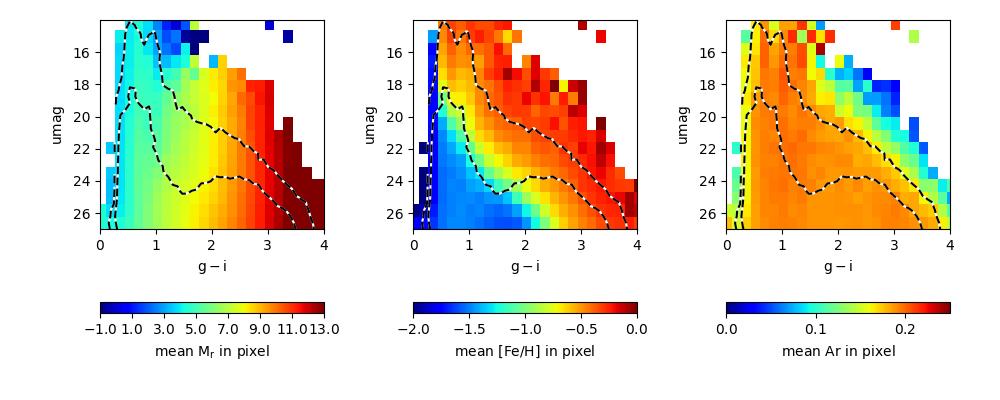
\includegraphics[width=1.08\textwidth,angle=0]{figures/qpBmeans_SDSSpatchRA340-350-simLSST_FeH.png}
\vskip -0.3in
\caption{The mean per-pixel values of absolute magnitude $M_r$, metallicity $[Fe/H]$, and interstellar dust extinction along the
  line of sight in the $r$ band, $A_r$, for a TRILEGAL-simulated sample of 280,000 main
  sequence and red giants stars with $r<26$, $u<27$, $340^{\degree} < {\rm R.A.} < 350^{\degree}$
  and $-1.3^{\degree} < \delta < 1.3^{\degree}$ (a small patch from the SDSS Stripe 82 region) in the $u$ vs. $g-i$
  color-magnitude diagram. The mean values are color-coded according to the legend below each panel. Contours
  visualize the sample distribution in each diagram. The strong variation of $M_r$ with the $g-i$ color is seen in the left panel,
  except for the small patch with $u<16.5$ and $1.0 < g-i < 1.5$ where red giant stars dominate. The
  diagonal iso-metallicity boundaries in the middle panel closely correspond to distance
  (in the range from about 1 kpc to about 100 kpc in the lower left corner). The values of
  dust extinction, shown in the right panel, are not large ($<0.2$) because the
  selected field is at high Galactic latitudes (centered on $b = -52^{\degree}$).}
\label{fig:qpBmeans}
\end{figure*}

Figures~\ref{fig:perfVSestParamsMr} and \ref{fig:perfVSestParamsFeH} show the summarized statistical performance of the Bayesian
method (bias, scatter, $\chi^2$) in the $u$ vs. $g-i$ color-magnitude diagram. In this test based on a high-galactic
latitude field, we assumed that all stars are beyond the dust layer and fixed $A_r$ to its known true value (in practice provided by dust
maps such as those from \citealt{schlegel_maps_1998}). When $A_r$ is considered as a free parameter in sky regions with small $A_r$,
the best-fit $A_r$ values are often underestimated for stars in the blue part of the stellar locus (because the reddening vector and locus
are nearly parallel; for more details, see \S2.7.1 in \citealt{2012ApJ...757..166B}). We note that at faint magnitudes probed by LSST, this
assumption will only break down very close to the Galactic plane.


 
\begin{figure*}[ht!]
\hskip -0.2in
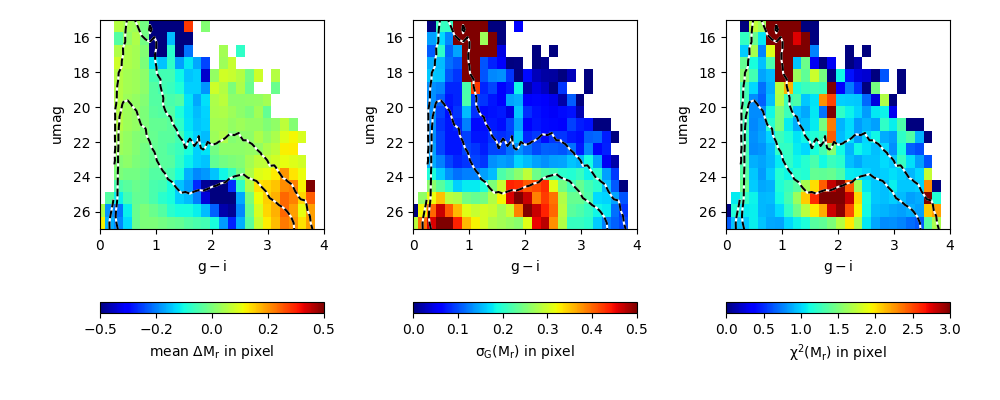
\includegraphics[width=1.06\textwidth,angle=0]{figures/qpB_estQ_SDSSpatchRA340-350-simLSST_Mr.png}
\vskip -0.3in
\caption{Statistical performance analysis for the estimates of model
  parameter $M_r$ (absolute magnitude), as a function of observed $u$
  band magnitude and the $g-i$ color, for the same simulated sample as shown
  in Figure~\ref{fig:qpBmeans}. 
  The left column shows the mean difference per pixel between the true
  and estimated values, the middle column shows scatter per pixel and
  the right column shows the scatter normalized by estimated
  uncertainties ($\chi^2$). Contours visualize the sample distribution in each
  diagram. Note that for main sequence stars $M_r>4$ and for most
  stars $4 < M_r < 10$. 
\label{fig:perfVSestParamsMr}}
\end{figure*}

\begin{figure*}[h!]
\hskip -0.2in
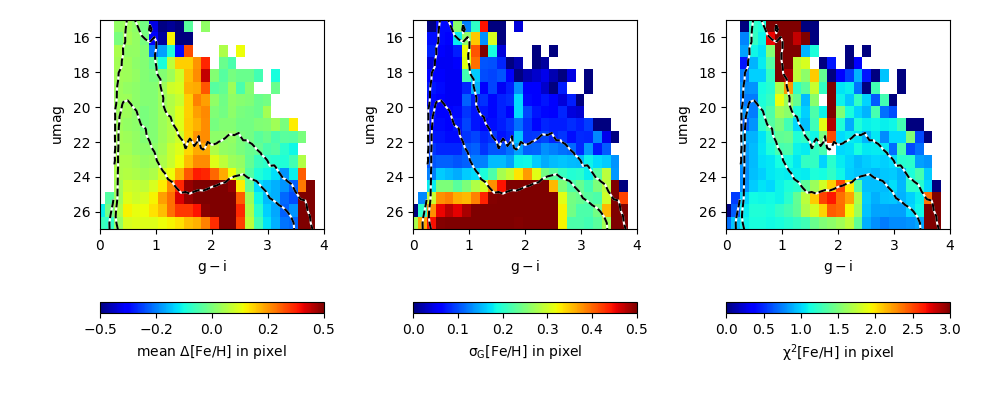
\includegraphics[width=1.06\textwidth,angle=0]{figures/qpB_estQ_SDSSpatchRA340-350-simLSST_FeH.png}
\vskip -0.3in
\caption{Analogous to Figure~\ref{fig:perfVSestParamsMr}, except for estimates of $[Fe/H]$ (metallicity) instead of $M_r$. 
\label{fig:perfVSestParamsFeH}}
\end{figure*}


As discussed in detail in \cite{2008ApJ...684..287I}, the photometric metallicity is best constrained for blue main-sequence stars with
$g-i<1$ (equivalently, $0.2 < g − r < 0.6$).
Therefore, we expect the best statistical behavior (smallest bias and scatter, $\chi^2 \sim 1$) in this color range, which is consistent with
the behavior seen in Figures~\ref{fig:perfVSestParamsMr} and \ref{fig:perfVSestParamsFeH}. An effective depth limit is about
$u=25$ (about 1 mag brighter than the 5-$\sigma$ depth in the $u$ band for coadded LSST photometry,  \citealt{2022ApJS..258....1B}); 
at fainter magnitudes the scatter between true and estimated values
for both $M_r$ and $[Fe/H]$ rapidly increases.

Figure~\ref{fig:perfVSestParams} shows a more quantitative illustration of the bias and scatter for best-fit $M_r$ and $[Fe/H]$ as
functions of the $u$ band magnitude, which sets the effective signal-to-noise ratio. In the bright limit ($u < 22$; approximately
$r<21$ for blue stars), $M_r$ and $[Fe/H]$ can be estimated with uncertainties of 0.10 mag and 0.07 dex, respectively, and essentially
negligible biases (0.02 mag for $M_r$ and 0.03 dex for $[Fe/H]$). These uncertainties are consistent with simulated photometric errors
and intrinsic properties of photometric parallax and photometric metallicity methods (for detailed discussion, see \citealt{2008ApJ...684..287I}). 

This $M_r$ uncertainty implies distance estimates for blue stars accurate to about 5\% to a distance limit of 25 kpc, with coadded LSST
photometry.  Such unprecedented accuracy for photometric distance estimates is due
to the ability of the $u$ band to constrain $[Fe/H]$. For a subsample with $u\sim24.73$, one magnitude brighter than 5-$\sigma$ limit,
the scatter increases to 0.27 mag and 0.38 dex, and further to 0.36 mag and 0.54 dex for a subsample at 5-$\sigma$ limit in the $u$ band
(where the $u$ band photometric uncertainty is 0.2 mag).  
 
As the right panel in Figure~\ref{fig:perfVSestParams} demonstrates, estimates of $M_r$ and $[Fe/H]$ are highly anti-correlated (this is essentially a
consequence of eq. A2 from \citealt{2008ApJ...684..287I}, also visible as the shift of stellar main sequence with metallicity in the top
panels in Figure~\ref{fig:augmLocus}). An $[Fe/H]$ uncertainty of 0.3 dex, approximately the width of the halo metallicity distribution, 
would induce an additional uncertainty of estimated photometric $M_r$ of 0.3 mag (as would be the case for faint stars with weak or no $[Fe/H]$ constraint
coming from their $u$ band measurement). 

The bias and scatter for both $M_r$ and $[Fe/H]$ are large in a small patch with $u<16.5$ and $1.0 < g-i < 1.5$ where red giant stars dominate,
due to strong degeneracies in color space between giants and main sequence stars (recall Figure~\ref{fig:RGdegeneracy}). 
About 2/3 of all red giants are mis-identified as main sequence stars (due to priors, as they are by and large indistinguishable by colors). 
Nevertheless, these simulation-based tests suggest that it will be possible to select highly pure samples of red giants using best-fit
$M_r$ and a simple $M_r < 3$ cut. This selection criterion selects 28\% of all red giants in the sample (which correspond to about 1\% of the full
sample), with a purity of 99.9\%. With LSST data, it will be possible to select such red giant candidates, if they exist, to
distances of several hundred kpc (note that low-$[Fe/H]$ main sequence stars at the blue edge of the stellar locus and $u=25$, with
LSST distance uncertainties of about 20\%, will be detected to distances of about 100 kpc).
 

\begin{figure*}[h]
\hskip 0.05in
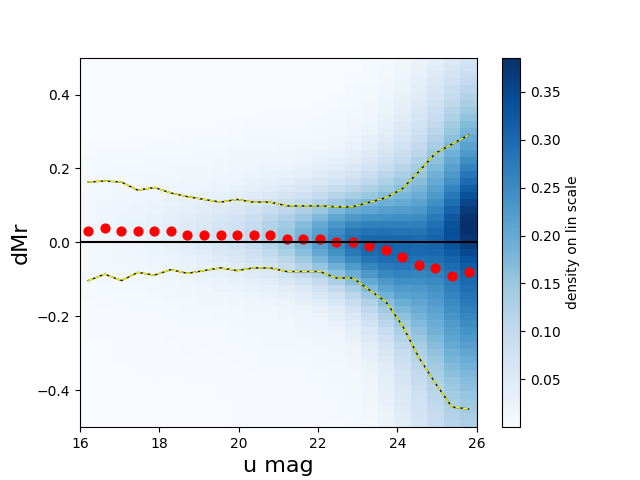
\includegraphics[width=0.35\textwidth,angle=0]{figures/dMrVSumag_SDSSpatchRA340-350-simLSST.png}
\hskip -0.12in
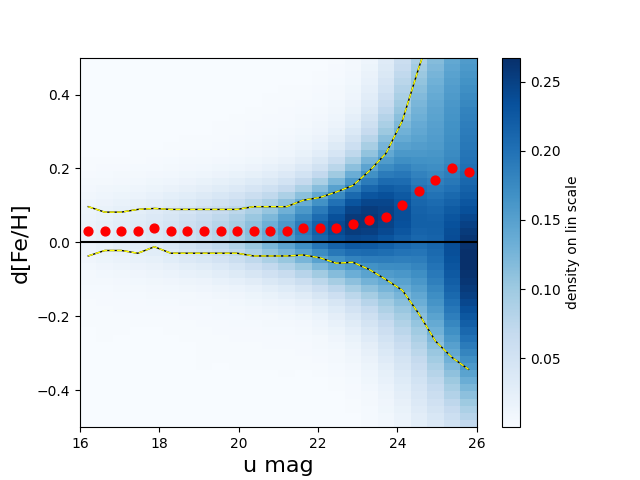
\includegraphics[width=0.35\textwidth,angle=0]{figures/dFeHVSumag_SDSSpatchRA340-350-simLSST.png} 
\hskip -0.12in
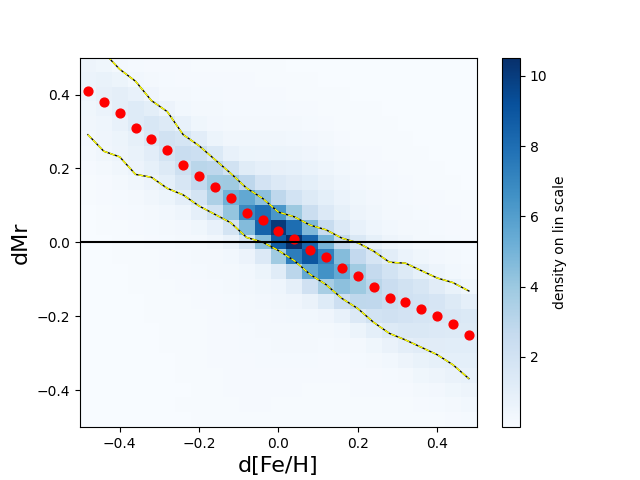
\includegraphics[width=0.35\textwidth,angle=0]{figures/dMrVSdFeH_SDSSpatchRA340-350-simLSST.png} 
\caption{The variation of the difference between the true and estimated values (left: $M_r$, middle: $[Fe/H]$) with $u$
  band magnitude. The binned background map shows the same simulated sample as in Figure~\ref{fig:qpBmeans}. 
  The symbols show binned medians and the dashed lines show robust standard deviation around the medians.
  At about $u=23$, the scatter for both $M_r$ and $[Fe/H]$ starts
  increasing due to increasing $u$ band measurement error. The dataset
  was generated assuming $u$ band 5-$\sigma$ limiting depth of 25.73
  for coadded LSST photometry  \citep{2022ApJS..258....1B}. 
  The right panel illustrates strong anti-correlation between the differences. 
\label{fig:perfVSestParams}}
\end{figure*}




\subsubsection{SDSS-based Comparison to Gaia's Distance Scale \label{sec:SDSSGaia}} 



\begin{figure*}[ht!]
\plotone{gaiaStripe82plot1.png}
\caption{Analysis of the difference between Gaia's geometric (trigonometric) absolute magnitudes and photometric magnitudes
  derived from SDSS colors. Symbols show a sample of 33,186 stars with the parallax signal-to-noise ratio above 10, absolute
  magnitude MrGeo$>$4 and MrPho$>$4 , and SDSS-based $u<21$ and $0.2 < g-r < 0.6$. The median magnitude difference is
  $-0.01$ mag, with a scatter of 0.28 mag. The four panel illustrate variation of the binned median (red circles) and scatter (red
  lines) with the $u$-band magnitude, the parallax signal-to-noise ratio, SDSS $g-r$ color, and photometric metallicity.} 
\label{fig:gaiasdss1}
\end{figure*}




\begin{figure*}[ht!]
\plotone{gaiaStripe82plot2.png}
\caption{Analysis of the difference between Gaia's photometric (color-based) absolute magnitudes and photometric magnitudes
  derived from SDSS colors. Symbols show a sample of 165,834 stars with absolute magnitude MrPho$>$4, and SDSS-based $u<21$
  and $0.2 < g-r < 0.6$. The median magnitude difference is $-0.05$ mag, with a scatter of 0.32 mag. The four panel illustrate
  variation of the binned median (red circles) and scatter (red lines) with the $u$-band magnitude, SDSS $u-g$ and $g-r$ colors,
  and photometric metallicity.}
\label{fig:gaiasdss2}
\end{figure*}



Analysis of the method's performance in the preceding subsection was based on a simulated sample with ``observed'' colors generated using
exactly the same luminosity-color model tracks as those used in fitting. Therefore, that analysis cannot test the validity of those tracks in an absolute sense.
While these empirical luminosity-color model tracks were derived using SDSS observations of
globular clusters with known distances and metallicities, here we validate them further using trigonometric distances recently obtained by Gaia.  

For validation, we used the SDSS Stripe 82 Standard Star Catalog, recalibrated by \cite{2021MNRAS.505.5941T},
which provides the most precise available photometry in SDSS bands (due to averaging of many repeated SDSS observations). 
For stars listed in the catalog, we extracted Gaia measurements and ``photogeometric'' distances from 
\cite{bailer-jones_estimating_2021}. Out of 841,000 stars listed in the Standard Star Catalog, there are 415,000 stars with $r < 22$, $u<22$ and a Gaia
match within 0.15 arcsec (after correcting for proper motion using Gaia measurements). Their distribution in color-color and
color-magnitude diagrams is shown in Figures~\ref{fig:3dataDiags} and \ref{fig:3HRdiags}. 
We estimated $M_r$ and $[Fe/H]$ for these stars using the same procedure and assumptions as for the simulated sample from the
preceding subsection. In particular, we assumed that all stars are beyond the dust layer and fixed $A_r$ to its value provided by the dust
maps from \cite{schlegel_maps_1998}.

We first analyze results for a subsample of stars that have $0.2 < g − r < 0.6$, a color range where photometric metallicity estimator is best constrained,
and a signal-to-noise ratio for Gaia's trigonometric
parallax measurement above 10.  We also required $u<21$ but that requirement is less stringent than the implied flux limit due to
Gaia's signal-to-noise ratio limit (approximately, $u<19$). There are about 18,000 stars in this subsample.
We find that their $M_r$ is estimated using SDSS photometry with a bias of 0.06 mag and root-mean-square scatter of 0.30 mag, compared
to Gaia's measurements. Equivalently, photometric distances  are estimated with a scatter of 15\% and a bias of 3\%.

The median contribution of Gaia's parallax measurement uncertainty to Gaia's absolute
magnitude uncertainty for this subsample is about 0.12 mag. This estimate implies that the median uncertainty of SDSS-based $M_r$
estimates is 0.27 mag (corresponding to about 14\% distance uncertainty). On the other hand, when only stars with signal-to-noise
ratio for Gaia's trigonometric parallax measurement above 50 are considered, the implied uncertainty of SDSS-based $M_r$
estimates is 0.21 mag (corresponding to about 10\% distance uncertainty).  Recalling that the statistical uncertainties for $M_r$
estimates using simulated sample in the preceding section are 0.10 mag at the bright end, these somewhat larger uncertainties may
imply additional statistical effects not accounted for in our analysis, and/or imperfect luminosity color-tracks.
Figure~\ref{fig:gaiasdss1} demonstrates that there are no concerningly large systematic errors in photometric $M_r$ estimates with
respect to photometric noise ($u$ band magnitude), $g-r$ color and photometric metallicity estimates (though note that the metallicity
range corresponds only to disk stars).

We extended our analysis to fainter magnitude limits by replacing Gaia's magnitudes based on trigonometric distance with those based on
the so-called ``photogeometric'' distances from \cite{bailer-jones_estimating_2021}. This comparison goes about 2
magnitudes deeper and also extends to low halo-like metallicity range. The scatter between photometric $M_r$ based on SDSS data and
$M_r$ based on ``photogeometric'' distances is 0.38 mag. As shown in Figure~\ref{fig:gaiasdss2}, the systematic error
increases to about 0.2-0.3 at the blue and low-metallicity edge of the stellar locus. When stars with $0.2 < g-r < 0.3$ are excluded,
systematic errors at the low-metallicity ($[Fe/H]<-1$) end disappear, indicating that it is the $M_r$ as a function of color relation that fails at the blue end,
rather than the shift of $M_r$ as a function of $[Fe/H]$. Such edge effects will have to be recalibrated when LSST photometry becomes available
(both using Gaia data and globular clusters). 



\subsubsection{Performance in the Galactic Plane}  

\begin{figure*}[ht!]
\hskip -0.2in
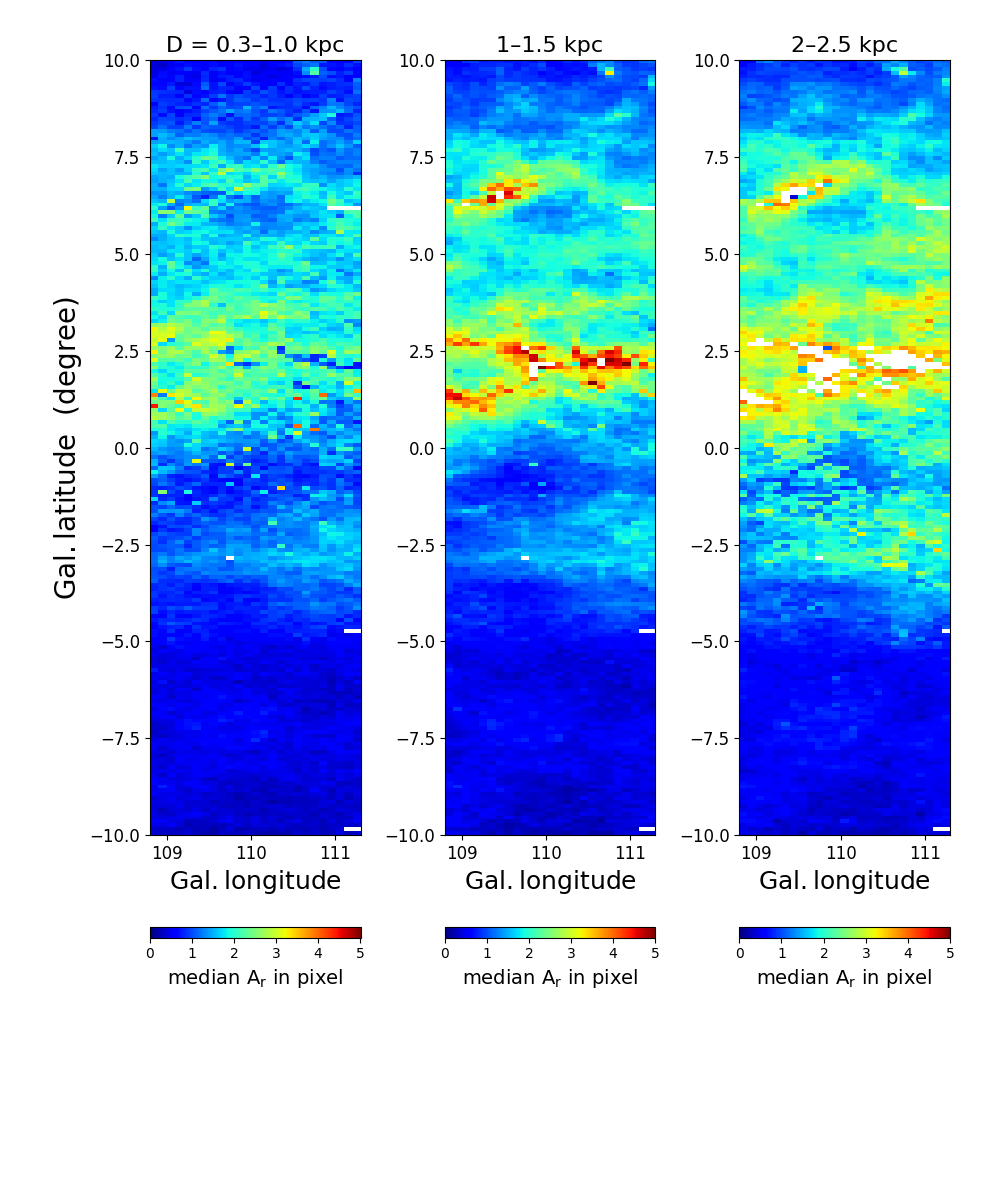
\includegraphics[width=1.06\textwidth,angle=0]{figures/qArSEGUEl110.png}
\vskip -1.4in
\caption{Color-coded maps show the best-fit $A_r$ (dust
  extinction along the line of sight) per pixel for the SDSS-SEGUE strip centered on $l = 110^{\degree}$
  (modeled after Figure~25 from \citealt{2012ApJ...757..166B}). Each pixel, defined in Galactic coordinates, shows the median Ar
  according to the legend below each panel.  The three panels  correspond to distance slices 0.3–-1 kpc (left), 1-–1.5 kpc (middle),
  and 2–-2.5 kpc (right). Note that the median extinction increases rapidly with distance. In the right panel, there are no stars in
  white regions in the center because extinction makes them fainter than the sample magnitude limit.
\label{fig:SEGUEdust}}
\end{figure*}


As the final test, we analyze the method's performance in regions with large interstellar dust extinction ($A_r$). We use SDSS-SEGUE data
collated and described by \cite{2012ApJ...757..166B}. For illustration, we use a single strip perpendicular to the Galactic
plane and centered on longitude $l=110^{\degree}$. Figure~\ref{fig:SEGUEdust} shows best-fit dust extinction along the
line of sight for three distance slices. Clear three-dimensional structure of the dust distribution is evident and consistent with
Figure~25 from \cite{2012ApJ...757..166B}.
 
These tests validate numerical implementation of the Bayesian algorithm and demonstrate its performance on a single patch of data, where priors
can be assumed uniform. An all-sky pipeline implementation is described in the next Section.
